%------------------------------------------------------------------------------
\hypertarget{lcap2}{}
\chapter{Sensor Fusion}
\vspace{-1cm} \label{cap2}

%\begin{flushright}
%\begin{minipage}{0.7\linewidth}
%\emph{``Quando uma criatura humana desperta para um grande sonho e
%sobre ele lan�a toda a for�a de sua alma, todo o universo conspira a
%seu favor.''}
%\end{minipage}
%\end{flushright}
%
%\begin{flushright}
%{Goethe}
%\end{flushright}

%\vspace{1cm}

%%Colocar uma descri��o do cap�tulo aqui!
%\section{Introdu��o}\label{sec int_cap_2}


In this chapter, we review sensor fusion techniques, advantages and terminologies. We start with a brief explanation on the motivations in this field of science, grouping them in two main categories: data authenticity and data availability. We continue with a definition of sensor fusion and an exploration of the available classification models for fusion methods. The categorization based on data challenges, that is imperfection, correlation, inconsistency and disparateness, is further discussed. We also present data fusion methods that handle imperfect data, which is the most fundamental problem present in information. We end the chapter focusing on probabilistic fusion methods for sampled-data systems.


\section{Contextualization}

The idea that combining information from multiple sensors to improve overall system performance has been in discussion for several decades. In the early days, there were those who argued against the synergism hype that was being spread in military systems, using the multi-sensor concept \citep{Fowler1979}. In his work, Fowler created what he called his seventh law: 

\begin{quote}
	"Be wary of proposals for synergistic systems. Most of the time when you try to make 2 + 2 = 5, you end up with 3... and sometimes 1.9"
\end{quote}

Although he was probably right to affirm that the added complexity and high costs are not always worth it - especially back then when devices were more expensive - many posterior studies advocated that the fusion of sensor data will always be better, in the sense that the probability of correctly classifying a target increases. However, such improvement depends on the condition that the statistical properties and characteristics of the uncertainty sources are properly known by the fusion process.

A direct answer to Fowler's work came in the year after with the publication of the work \citep{Nahin1980}, when Nahin and Pokoski used strict concepts and definitions to prove that the addition of sensors improves network performance, but also acknowledged their assumptions of discarding complexity and costs for the sake of their arguments. This topic continued to draw scientific attention throughout the years, like the work of \citep{Rao1998} and \citep{Dasarathy2000}. Rao focused on fusion methods and its comparison to classifiers' performance. He also established conditions that guaranteed that the fused system will at least perform as good as the best classifier. Dasarathy's work extended that of Rao's, but it was able to describe a certain scenario at which a two-sensor scheme outperforms a three-sensor architecture from a parametric fusion benefits domain perspective. In order to compare performances of fusion levels or algorithms and assess possible benefits of sensor fusion, \citep{Theil2000} discussed three measures of performance, one for each sensor management process, which are detection, tracking and classification.

Despite all philosophical discussions, many real applications have been taking advantage of sensor fusion benefits since its advent, like remote sensing \citep{Foster1981}, robotics \citep{Richardson1988} and intelligent systems \citep{Luo1989}. Recently, with the modernization and popularization of sensors, its use has grown significantly, with hot topics emerging in the area, such as body sensor networks for health-care applications \citep{Gravina2017}, artificial intelligence \citep{Safari2014, Jordao2018} and smart grids \citep{Liu2012, Kordestani2017}. Recent reviews of the state of the art \citep{Khaleghi2013, Jing2013} provide a very broad understanding of the field and its advances. 

\section{Motivation and Advantages}\label{sec:motivation}

Whether or not all sensor fusion approaches outperform the use of less sensors in every aspect for any given condition, the fact is that many fields of science and engineering have been benefiting from choosing the fusion approach.

The reasons why one chooses to fuse information from different sources are various. The works of \citep{Hall1997, Elmenreich2002, Andler2009, Khaleghi2013} provide a detailed study on the motivations and advantages of multi-sensor data fusion techniques. A common benefit from the use of multiple redundant sensors, for instance, is the increase in accuracy. By averaging all the measurements, the expected error decreases by the rate of $(\sqrt{n})^{-1}$, where $n$ is the number of homogeneous sensors, in case of the presence of i.i.d Gaussian noises. In Figure \ref{fig:accuracy} different probability density functions (PDFs) with different standard deviations - thus different uncertainty levels - are shown for various quantities of random variables being averaged.

\begin{figure}[!htb]
	\centering
	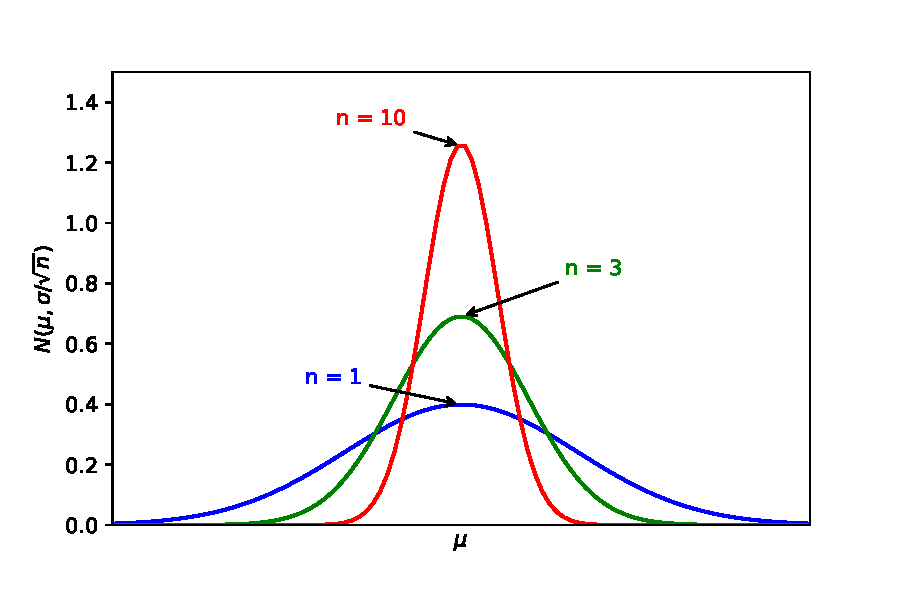
\includegraphics[width=0.8\textwidth]{Imagens/fusion_accuracy.pdf}
	\caption[PDFs for different amount of fused measurements]{PDFs for different amount of fused measurements, obtained by 1 (blue), 3 (green) and 10 (red) redundant sensors, considering i.i.d additive Gaussian noise. The higher the value of $n$, the lower is the standard deviation.}
	\label{fig:accuracy}
\end{figure}

%There are many other reasons to fuse information from multiple sensors. \citep{Elmenreich2002} provides an interesting example to illustrate some of them. Imagine a car parking assist system with only one distance sensor mounted at its rear, with limited precision and considerable update time (sampling interval). Now picture how would be the system's performance, considering that the sensor may suffer from: deprivation or occlusion, in the sense that it could be blocked by some physical barrier; coverage, both in spatial and temporal contexts, since it can only sense objects in front of him (spatial) and can only provide information periodically (temporal); precision, with measurement errors being liable to be the cause of unexpected bumps; and uncertainty, when an object, such as a small bicycle, might be missed by the sensor even in the presence of valid signal. The system would definitely perform at insufficient levels. All these issues could be solved by adding multiple sensors to the architecture.

%%%% CORRIGIR EM CASO DE TROCA DE ORDEM

There are many other advantages to fusing information from multiple sensors. Based on the studies by Hall, Elmenreich and Andler, we can group most of them in two categories: \emph{authenticity} and \emph{availability} improvements. The first group refers to those benefits that improve the quality of the measurement, whereas the second one encompasses those benefits regarding ranges or data dimensions. The set of multiple sensors can also be of different types (\emph{heterogeneous}), or of the same type (\emph{homogeneous}), with redundant measurements. There may be benefits that are exclusive to the addition of different sensors, others exclusive to the addition of redundant sensors and those that can happen both ways. Figure \ref{fig:advantages} presents a schematic with the different advantages expected in sensor fusion.

\begin{figure}[!htb]
	\centering
	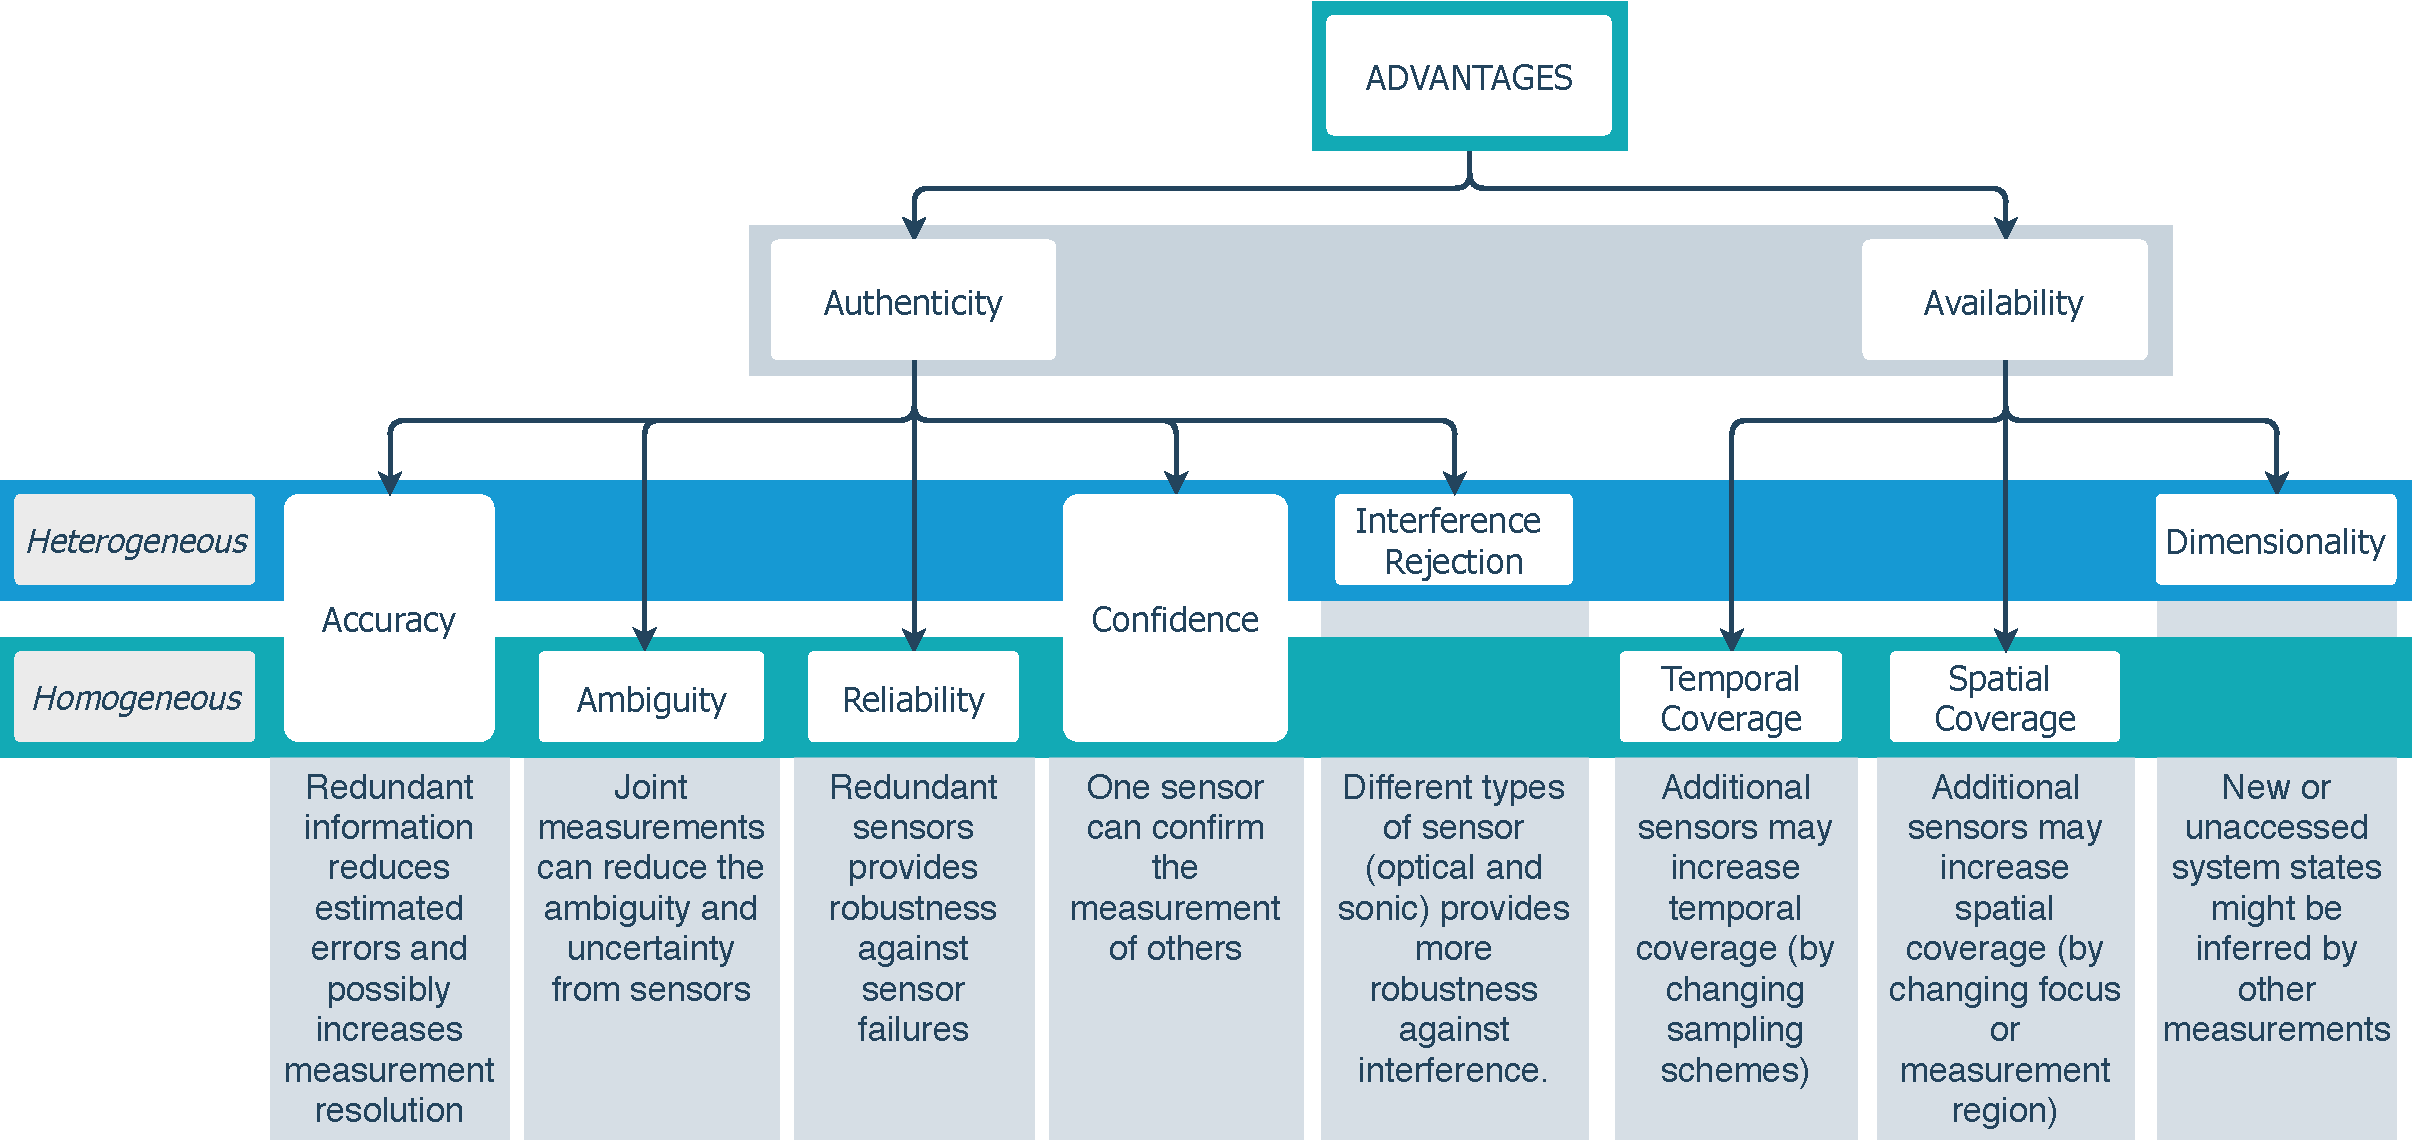
\includegraphics[width=\textwidth]{Imagens/fusion_advantages.pdf}
	\caption[Expected advantages in sensor fusion]{Sensor fusion categorization hierarchy based on expected advantages. The white boxes represent the advantages grouped two ways: between autenthicity or availability improvements; and between heterogeneous, homogeneous or both sensor architectures}
	\label{fig:advantages}
\end{figure}


\section{Taxonomy and Classification}\label{sec:classification}

Sensor fusion definitions have evolved throughout the years. The work of \citep{Bostrom2007} analyses more than 30 papers on this matter, to propose a more comprehensive and precise definition to the broad area of information, data and sensor fusion, which we reproduce here:

\begin{quote}
	"Information fusion is the study of efficient methods for automatically or semi-automatically transforming information from different sources and different points in time into a representation that provides effective support for human or automated decision making."
\end{quote}

Researchers in the field made additional efforts to categorize the fusion techniques, using different approaches. One of the earliest attempts comes from \citep{Durrant1988}, where he considered the dynamic use of information in the fusion processes, creating the so-called dependence model, which grouped sensor fusion in three categories: \emph{competitive}, \emph{complementary} and \emph{cooperative}. Competitive type occurs when multiple sensors measure the same properties, usually referred to as redundant architecture. Complementary fusion describes the scheme of different types of sensors measuring different information about the same global object or feature, enabling a more complete fused information, like multiple cameras covering a large area. And the last category, cooperative fusion, happens when more complex data are combined to provide information that would not be available (or hard to obtain) otherwise. An example would be multiple measurements being processed to create soft sensors. An illustrative schematic is presented in Figure~\ref{fig:cat_input}. An abstraction from the human sensory system to Whyte's model can be done by understanding the way flavors are perceived by our taste and smell sensors, tongue and nose, respectively, in a cooperative fashion, while our both eyes or our both ears perform some sort of complementary fusion. 

\begin{figure}[!htb]
	\centering
	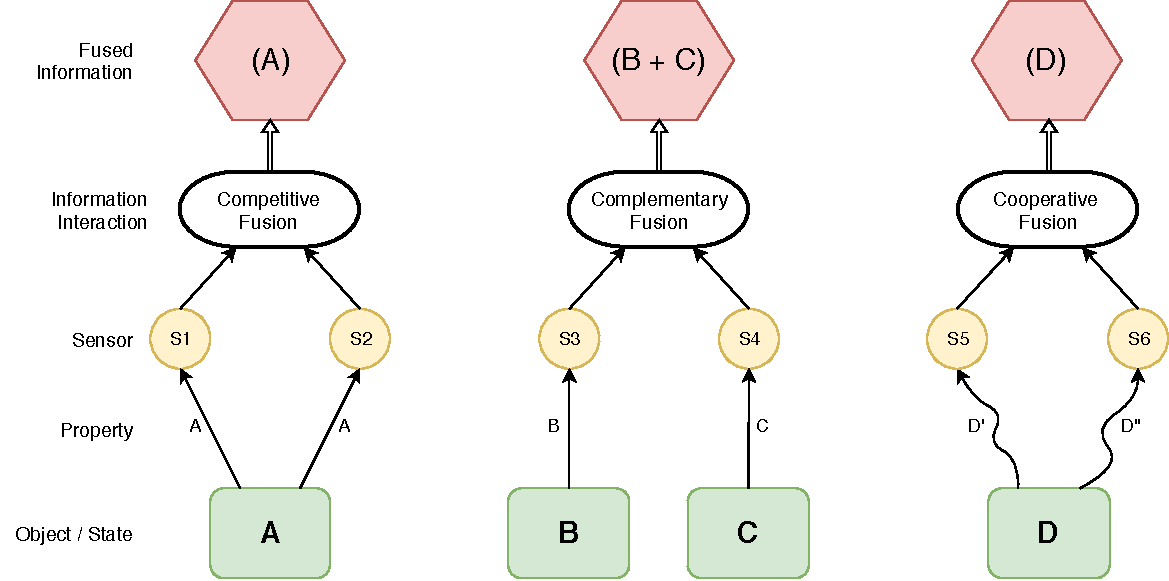
\includegraphics[width=\textwidth]{Imagens/fusion_cat_input.pdf}
	\caption[Classification of data fusion based on sensor interaction.]{Classification of data fusion based on sensor interaction. The lower green boxes represent the states or objects being measured. Their properties can be observed directly (straight lines) or indirectly (curved lines) by sensors indicated by the letter S. After fusion, the output information is presented in the red hexagons. Adapted from \citep{Elmenreich2002}.}
	\label{fig:cat_input}
\end{figure}

Another common way to categorize sensor fusion is by the \emph{three-level hierarchy} based on input and output characteristics, which depends on the processing stage at which information is fused. The lower-level is related to \emph{raw-data fusion}, where signals from sensors are combined. The mid-level is usually related to \emph{feature fusion}, where information about characteristics of the object are used in the process. The higher level involves \emph{decision fusion}, that can be understood as a reasoning process, like the methods of evidential belief or fuzzy logic. \citep{Dasarathy1997} extended this terminology, proposing five fusion modes, according to Figure~\ref{fig:cat_io}. \textit{Data in - data out fusion} (DAI-DAO), the lowest level fusion, processes raw data and outputs raw data, but with some improvements, such as increased accuracy. \textit{Data in - feature out fusion} (DAI-FEO) extracts features from raw data to describe characteristics of the measured environment. \textit{Feature in - feature out} (FEI-FEO) aims at the refinement of the features entering the process, similarly to what DAI - DAO does to raw data. \textit{Feature in - decison out} (FEI-DEO) usually performs classification based on a set of features received as inputs. \textit{Decision in - decision out} (DEI-DEO) outputs a better global decision based on local, restricted decisions. Using our human brain data fusion analogy, many examples can be framed into Dasarathy's terminology. The processing of raw signals, such as letters symbols, into features such as words and texts can be interpreted as DAI-FEO fusion. On the other hand, the process of assimilating features of objects from our eyes and ears, and fusing them into a decision about what they are, for instance, can be perceived as an example of FEI-DEO fusion.


\begin{figure}[!htb]
	\centering
	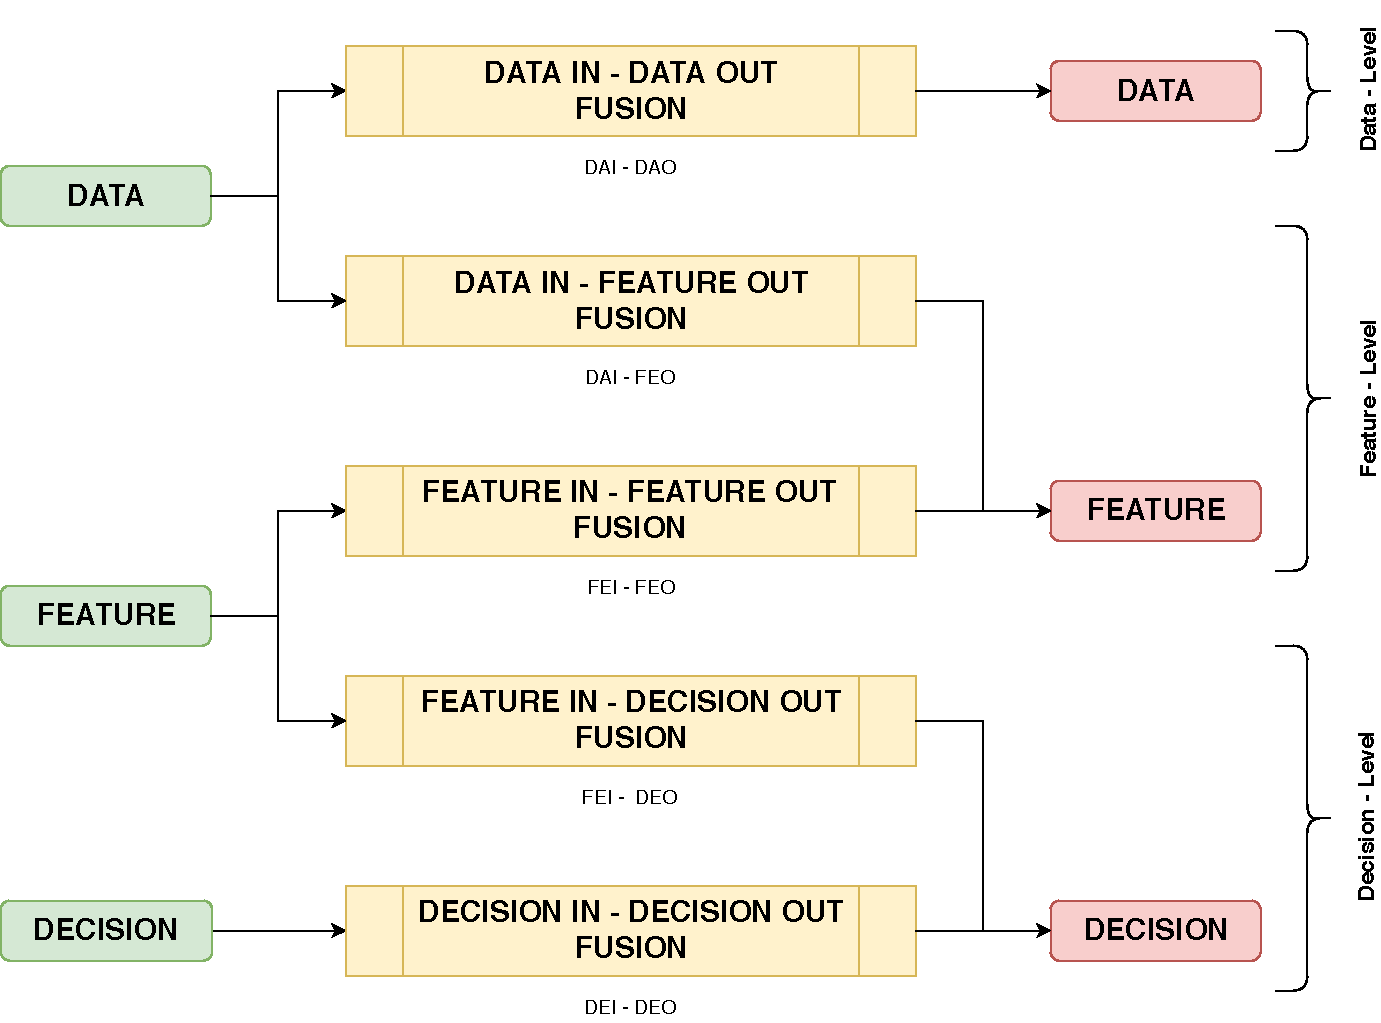
\includegraphics[width=\textwidth]{Imagens/fusion_cat_io.pdf}
	\caption[Input and output model and the three fusion levels.]{Input and output model categorization, representing type of input in green, the method in yellow and the output in red. The fusion levels are shown in the curly brackets. Adapted from \citep{Dasarathy1997}}
	\label{fig:cat_io}
\end{figure}

The work of \citep{Castanedo2013} provides a comprehensive review of these and other classifications of data fusion techniques. His efforts went beyond as he proposed an interesting new approach, based on the type of architecture, summarized in Figure~\ref{fig:cat_arch}. In his model, fusion techniques that collect all measurements in a central processor lie on the \emph{centralized} architecture category. Assuming perfect data alignment and association, such scheme should be optimal. However it is keen to many sampling irregularity related issues and might provoke network congestion. When a network of nodes is used, each with its own processing capability, the architecture becomes \emph{decentralized}. Such modular strategy ensures scalability, since there are no limits to centralized bottlenecks, and survivability to the loss of a particular sensing node. However it can greatly increase communication costs. The third and last configuration is the \emph{distributed} architecture, where each data association is performed by local nodes. The separate outputs are then transmitted to a fusion node, that processes these locally obtained estimates to produce a fused global estimate. This scheme will reduce both the communication costs from decentralized architecture and computational costs from the centralized one, while lacking some of their benefits. A fourth architecture could be defined as \emph{hierarchical}, which combines decentralized and distributed schemes, performing fusion at multiple levels. Getting back to our human sensory capacity, a very complex hierarchical architecture would best describe our brain fusion scheme in Castanedo's classification.

\begin{figure}[!htb]
	\centering
	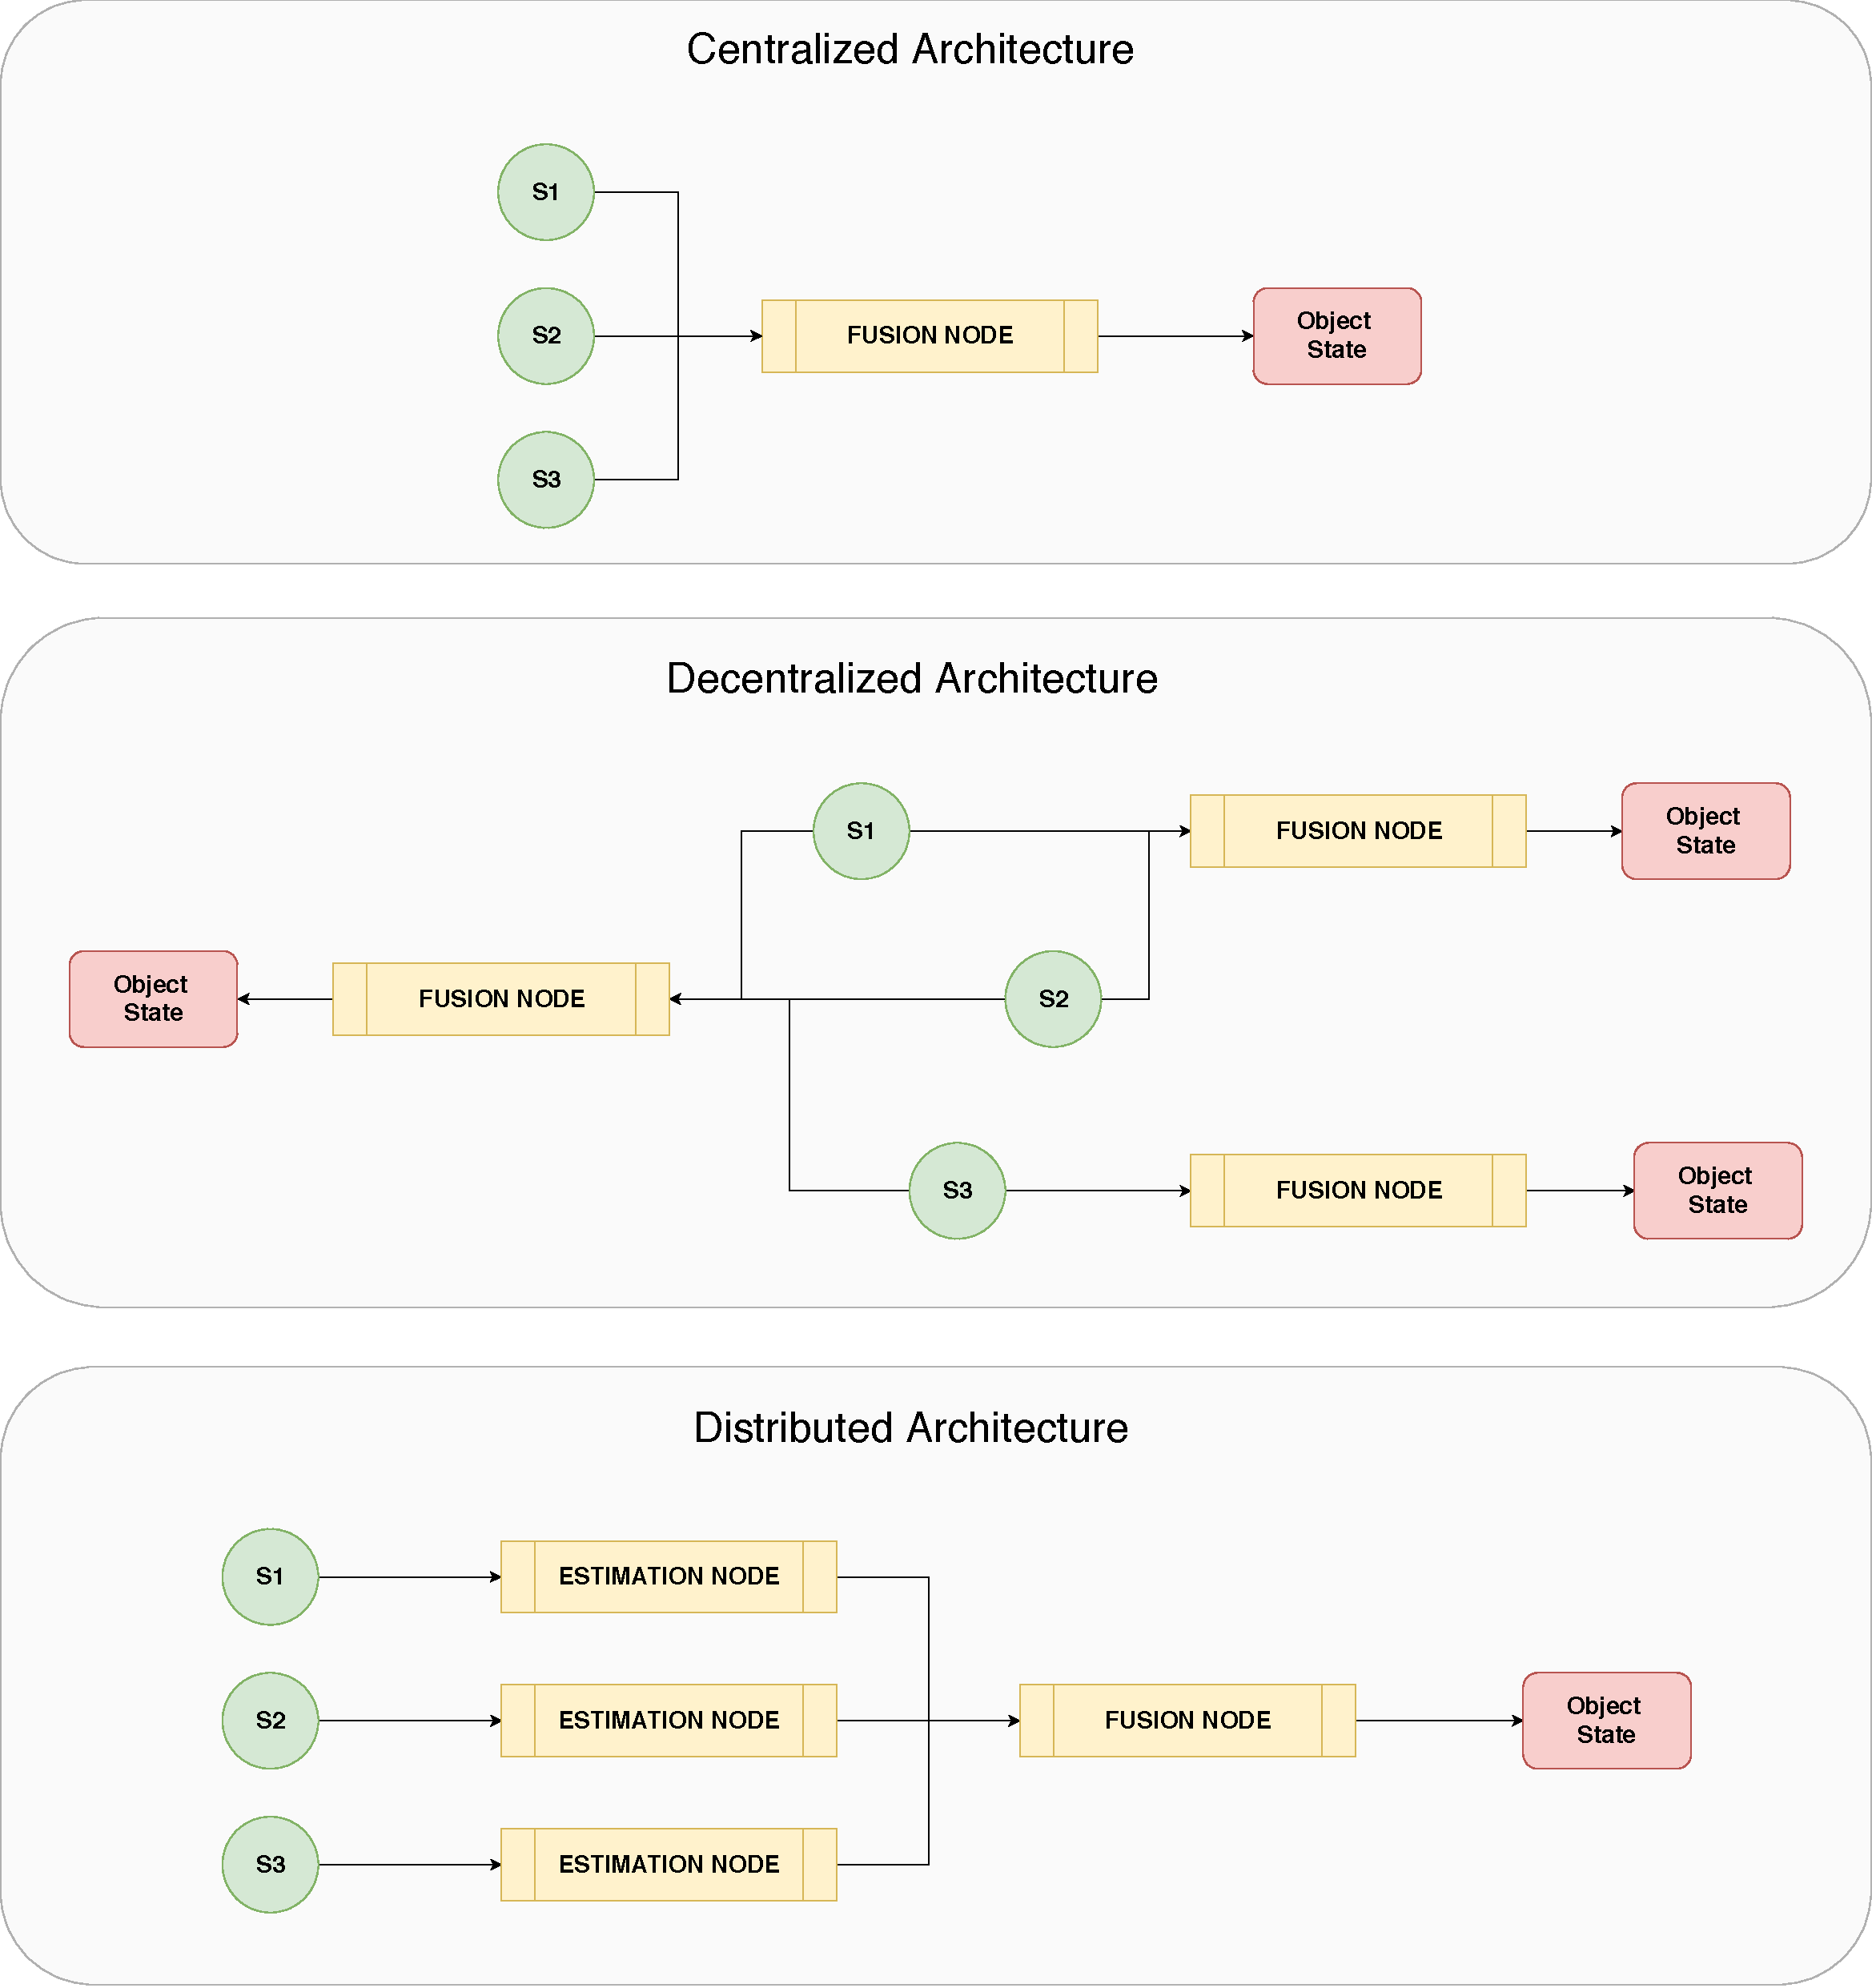
\includegraphics[width=\textwidth]{Imagens/fusion_cat_arch.pdf}
	\caption[Sensor network architectures for data fusion.]{Sensor network architectures for data fusion: \emph{centralized}, \emph{decentralized} and \emph{distributed}. Sensors are shown in green circles and the arrows represent the information flow. Adapted from \citep{Castanedo2013}}
	\label{fig:cat_arch}
\end{figure}

A final note on the taxonomy of data fusion methodologies will be given considering the work of \citep{Khaleghi2013}, due to its connections to sensor fusion in the presence of irregularities, like the ones that we discuss in Chapter \ref{cap3}. The idea was to study the methods based on data characteristics that make data fusion a challenging task. The authors referred to these aspects of data as data-related challenges and categorized the methods by which challenges the methods address. An overview of the challenge hierarchy proposed by the authors is presented in Figure~\ref{fig:fusion_challenge}, with four main categories of how challenging input data can be: \emph{imperfect}, \emph{correlated}, \emph{inconsistent} and \emph{disparate}. The most fundamental problem present in data is imperfection, an issue explained in details in Section~\ref{sec:impefect}. Indeed, most of the algorithms framed in the other three categories are basically methods that try to neutralize, avoid or minimize their aspects, so that imperfection is the only thing left on data. When correlation is present on data, for instance, the requirements for typical fusion algorithms, such as the Kalman Filter, are broken, so there are methods to eliminate correlation or to minimize its effects, given certain assumptions. In case of data inconsistency, due to outliers, one can act on the sensor outputs directly, to validate information or to detect and remove them automatically. If there are out-of-sequence measurements (OOSM) in data, a type of inconsistency, then the usual frameworks would be: to ignore; to reprocess or use backward/forward prediction; and to augment the state matrices in order to incorporate delayed measurements. Conflicted and disparate data are more specific and are beyond the scope of this study.

\begin{figure}[!htb]
	\centering
	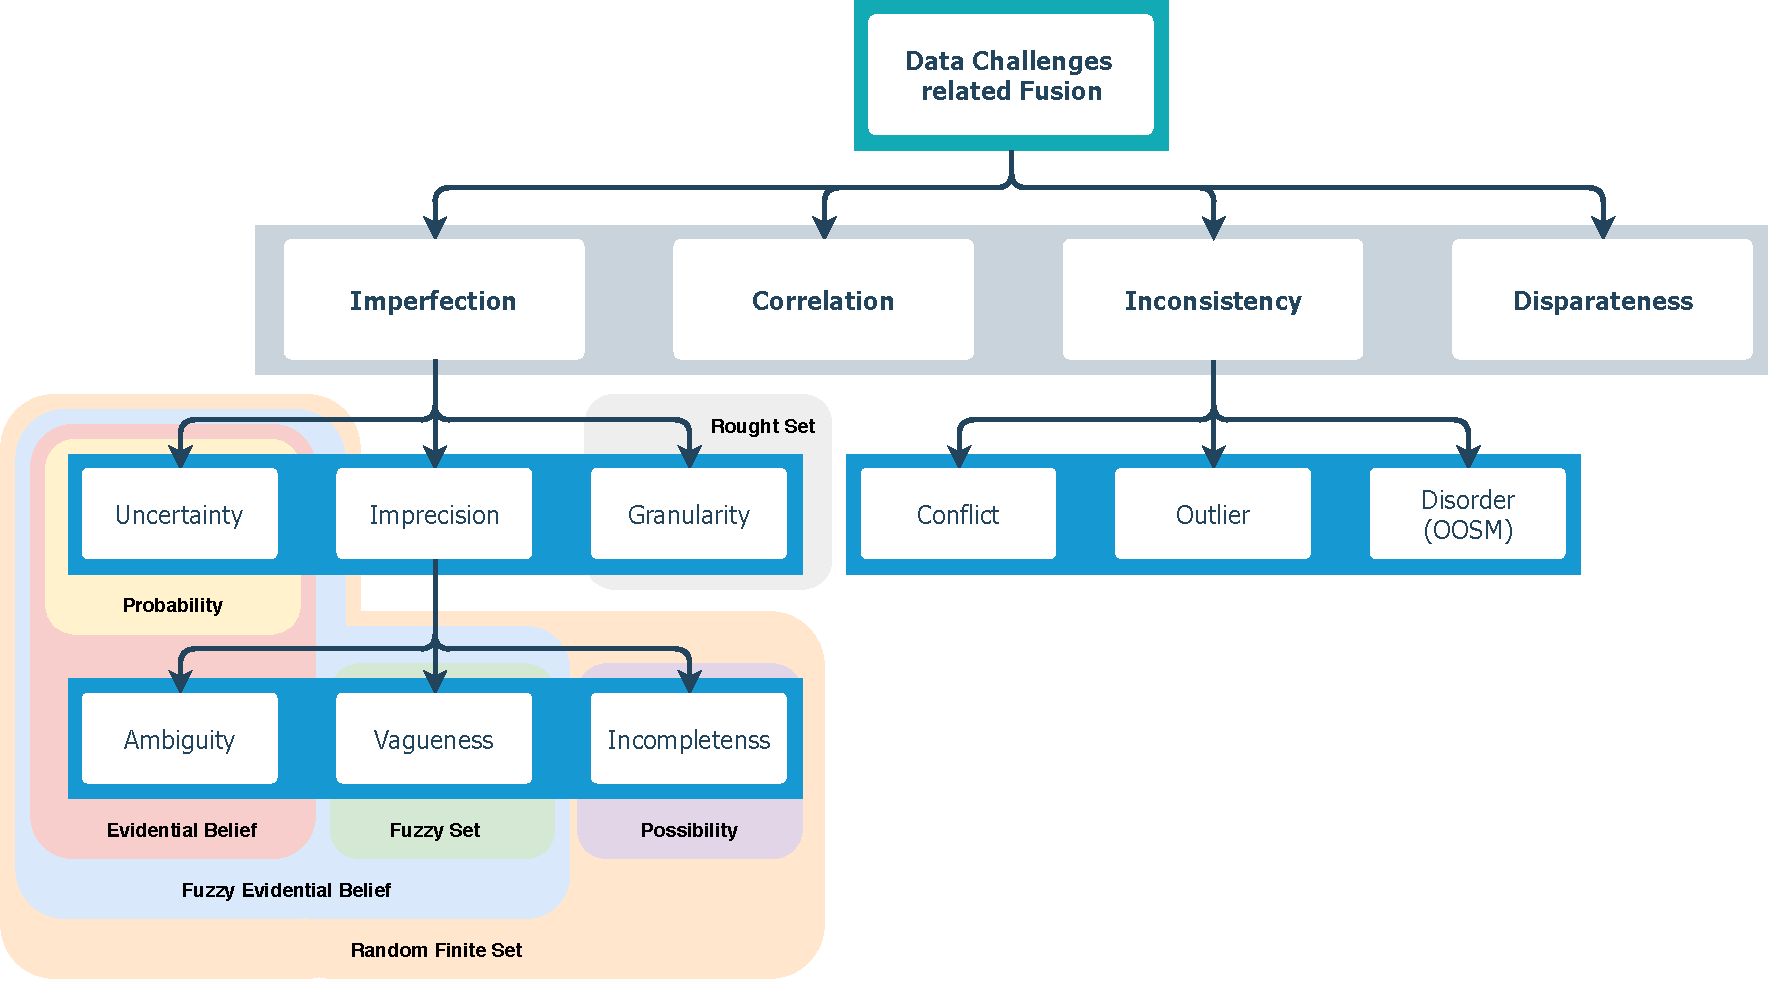
\includegraphics[width=\textwidth]{Imagens/fusion_challenge2.pdf}
	\caption[Data fusion categorization based on data challenges hierarchy]{Categorization based on data challenges hierarchy. For imperfect data, fusion methods and the issues they deal with are also presented. Based on \citep{Khaleghi2013}}
	\label{fig:fusion_challenge}
\end{figure}


\section{Approaches for the Fusion of Imperfect Data}\label{sec:impefect}

Being the most fundamental and common challenge present on data, imperfection is also the main focus for research in the area. Based on Khaleghi's classification, imperfection on data can be manifested as uncertainty, imprecision and granularity. We can distinguish uncertainty and imprecision with two information examples: \textit{I believe Maria is one point eight meter tall}; \textit{I am sure that Maria is tall}. In the first sentence, the information is precise, but uncertain. In the second, the information about Maria's height is certain, but imprecise, with some vagueness (fuzziness) attached to it. Usually the amount of precision in data is inversely proportional to the level of certainty. A source of imprecision can also be ambiguity, as in the phrase: \textit{Maria gave birth to her daughter yesterday at 5}. We don't know if it was 5 PM or 5 AM, though the information was certain. The last type of imprecision would be for incomplete data, when we have missing information. The sentence "\textit{Maria's height is above one point five meter}", is incomplete, for example, meaning that only one bound was given. Any height above one hundred and fifty centimeters is possible and any height less than or equal to it is impossible, defining the so-called possibility measures. Finally, granularity is an imperfection related to the internal structure of data, referring to the capacity of distinction among states. Different attributes on the data or a different set of possible states will generate different levels of imprecise information.

Given the amount of potential problems in data and their particularities, it is only natural that no data fusion approach alone could tackle all of them. Researchers have proposed various approaches that focus on one or a few of these issues and \citep{Khaleghi2013} explore methods for all the challenges in their categorization model. In this study we will limit ourselves to imperfect data, for which, in most cases, the mathematical background of the algorithms relies on the representation of imperfection. These methods are highlighted in Figure~\ref{fig:fusion_challenge} in different colors and covering one or multiple aspects. In the next subsections we will explore them. Table~\ref{tab:methods} presents a summary of all methods with their main advantages and limitations, adapted from the study of Khaleghi and his coauthors.
\vfill
\subsection{Probabilistic}

Uncertainty is the most natural source of data imperfection and it is usually modeled by probability density functions (PDFs). Thus, probabilistic fusion methods are the most adequate to handle it. The most classical approach to fuse data based on uncertain measurements is using Bayes' theorem. The idea is to update the probabilities of an hypothesis $H$ given some evidence $E$ by using the famous equation~\citep{Stone2013}

\begin{equation}\label{eq:bayes}
\rho(H|E) = \frac{\rho(E|H) \rho(H)}{\rho(E)},
\end{equation}

\noindent
where $\rho(H|E)$ represents a conditional probability, that is the probability of $H$ being true, given $E$. We can interpret (\ref{eq:bayes}) as a fusion of \textit{a-priori} belief of an hypothesis ($\rho(H)$) and the normalized likelihood of the evidence ($\rho(E|H)/\rho(E)$) to obtain a better current estimate of the hypothesis ($\rho(H|E)$). 

In addition to Bayes' contribution, Gauss' least squares methods and Fisher's maximum likelihood estimation are the foundations of all probabilistic approaches to data fusion, recursive filtering and state estimation. \citep{Kolmogorov1962} in 1941 and \citep{Wiener1949} in 1942\footnote{Their discoveries went public a few years later due to secrecy during war times.} independently designed a linear minimum mean-square estimation technique that is considered to be the first probabilistic designed filter, the so called Wiener-Kolmogorov filter. A few years later, perfecting the work of its predecessors, \citep{Kalman1960} developed the recursive mean-square filter, a groundbreaking method known as Kalman Filter (KF). Its impact was so big, that only one year after its publication, Kalman's algorithm was used in the Apollo Project \citep{Mohinder2010} to solve its guidance and navigation problem. A review on the evolution of least-squares estimation theory is provided by \citep{Sorenson1970}.

When it comes to a multi-sensor system, \citep{Willner1976} introduced three approaches for the discrete Kalman Filter: parallel, sequential and data compression filters. In the parallel filter, all measurements are processed by a KF in parallel, producing a multi-output estimation. For the sequential filter design, multiple KFs are used, where the estimates of a predecessor KF are used as input for the successor KF. Data compression or output fusion filter design compresses similar data using their noise covariance matrix beforehand and the fused output is used as the measurement for a single KF. A fourth method was proposed by \citep{Singer1971}, referred to as track-to-track fusion (TTF), that employs single-output KFs and fuses their outputs considering the correlation between them.

\subsection{Evidential Belief}
A different framework for managing imperfection is based on Dempster-Shafer evidence theory (DSET) \citep{Shafer1976}. Shafer argued that his theory, extended from Dempster findings, includes the Bayesian approach as a special case of evidence combination or information fusion. The difference between both relies on the assignment of uncertainty. Whereas Bayesian framework considers one multi-variable PDF to represent each state's uncertainty and the respective covariances, evidential belief theory assigns uncertainties not just to the states, but also to all its possible subsets, using probability mass functions. Imagine the example of Maria giving birth and the information about the time it happened. We can assign uncertainties to the ambiguous possibilities "5 PM" and "5 AM", in order to use the data. If the uncertainty about the information was also an aspect of the data, evidential belief approach could handle it likewise.

Therefore, DSET can be more adequate when fusion takes place at a higher-level estimation, that is the decision-level, referring back to the input and output classification model from Figure~\ref{fig:cat_io}. Situations related to risk assessment configure classical applications \citep{Srivastava2011}, where we have features or local decisions as inputs, usually with ambiguous and conflicting information and we need to take a global decision out of it. 

\subsection{Fuzzy Logic}\label{sec:fuzzy}

Fuzzy logic, first proposed by \citep{Zadeh1965} is a well known to handle vagueness in information. Unlike classical crisp definitions, where an element $x$ belongs or not to some set $A$, fuzzy sets are characterized by a \textit{membership function} $\mu_A(x)$ which associate values between 0 and 1 with the degree to which a given object $x$ belongs to a set $A$. That is, the closer $\mu_A (x)$ is to the one, more certain we are that $x$ belongs to $A$. For example, instead of defining tall people as those with height above certain crisp lower bound, we can define a membership function that assigns continuous degrees of "tallness" to different people. Zadeh also generalized the crisp set notion of operations to the fuzzy set theory: fuzzy complements (NOT), fuzzy intersections (AND) and fuzzy unions (OR).

Vague data can then be fused using fuzzy inference systems (FIS), mapping input variables into an output space using fuzzy logic operators through a set of If-Then fuzzy rules. One of the most widely used FIS are the Mamdani-type \citep{Mamdani1975} and Sugeno-type \citep{Sugeno1985}. The main difference between both is that the outputs of the former rules are also a fuzzy set, while the outputs of the latter rules are functions of the input variables. Mamdani and Sugeno-type rules are given, respectively, by
\begin{align}
R_i^{Mamdani} &: \textrm{If } x_{1} \textrm{ is } A_{i,1} \textrm{ and } x_2 \textrm{ is } A_{i,2}\textrm{ ... and } x_{n} \textrm{ is } A_{i,n} \textrm{, Then } y_i \textrm{ is } C_i, \\
R_i^{Sugeno} &: \textrm{If } x_{1} \textrm{ is } A_{i,1} \textrm{ and } x_2 \textrm{ is } A_{i,2}\textrm{ ... and } x_{n} \textrm{ is } A_{i,n} \textrm{, Then } y_i \textrm{ is } f_i(X),
\end{align} 

\noindent
where $x_j \in \mathbb{R}$ $\forall j = 1\textrm{,...,}n$, is the $j^{\textrm{th}}$ input variable, $A_{i,j}$ is the $j^{\textrm{th}}$ antecedent fuzzy set for the $i^{\textrm{th}}$ rule, $C_i$ is the consequent fuzzy set for the $i^{\textrm{th}}$ rule, $f_i(X)$ is the function of the input vector $X$. 

Therefore, we can understand the inference process as a series of steps, according to Figure~\ref{fig:fuzzy}. First, we fuzzify the inputs via membership functions. Then we apply the logic operators defined by each rule and find the result implications as the consequents. Finally we aggregate the consequents accross all rules and defuzzify its result. 

\begin{figure}[!htb]
	\centering
	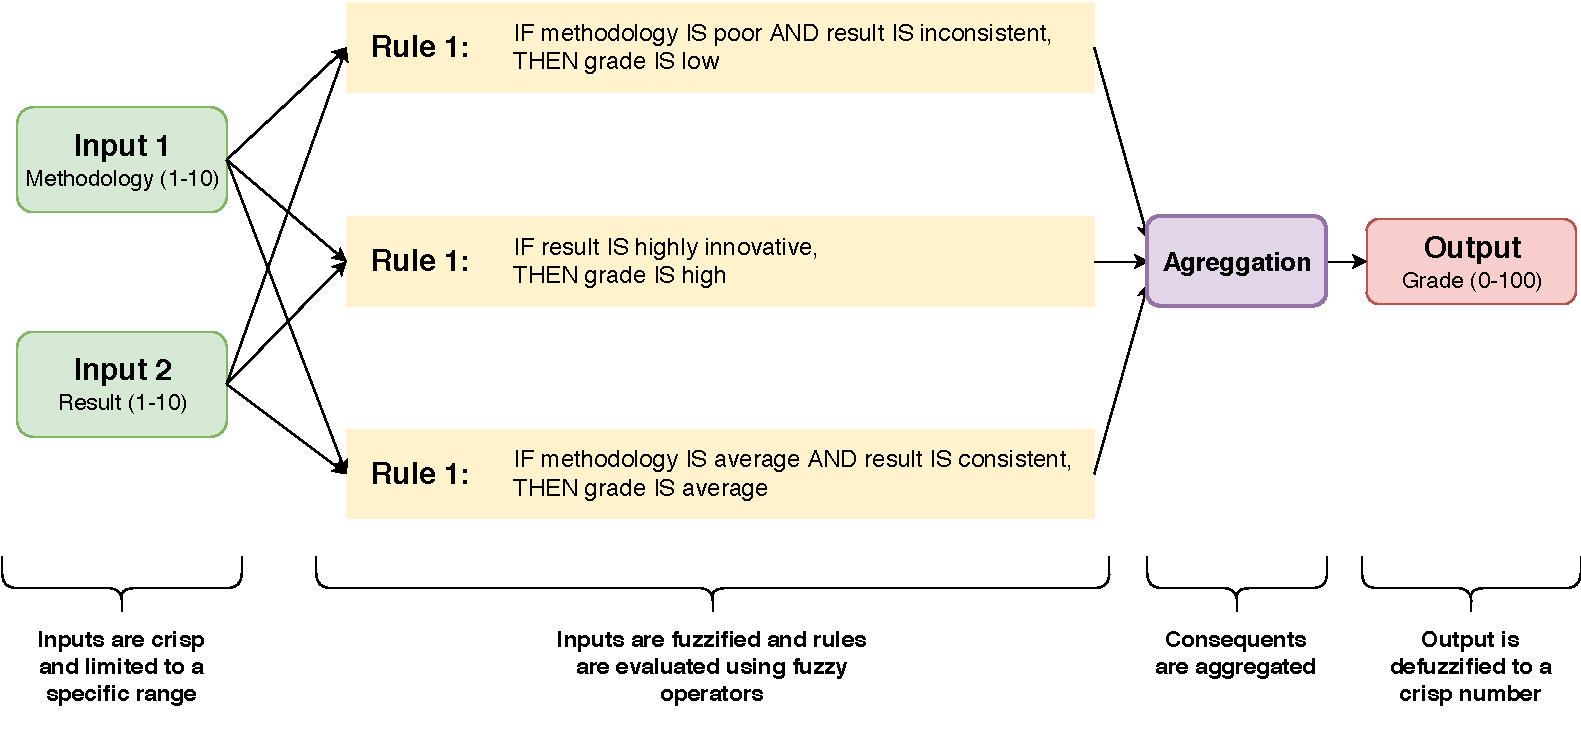
\includegraphics[width=\textwidth]{Imagens/fusion_fuzzy.pdf}
	\caption[Fuzzy inference system example]{Fuzzy inference system example for grading thesis. There are two inputs: methodology and result. They are fuzzified according to the antecedent membership fuzzy sets: poor and average for methodology; and inconsistent, consistent and highly innovative for result. After evaluation of the rules, the implication on the consequents are calculated, producing output fuzzy sets, that are finally aggregated. The final output is then defuzzified to produce a crisp number for the grade, between 0 and 100.}
	\label{fig:fuzzy}
\end{figure}


Fuzzy set theory differentiates itself from probabilistic and evidential reasoning theories by modeling the fuzzy membership of a state whose class is ill-defined, whereas the other methods model uncertainties in well-defined state classes.

It is possible to combine fuzzy theory with DSET to handle the imperfections that both approaches can deal with, that is uncertainty, ambiguity and vagueness all together, using the fuzzy evidential belief framework \citep{Yen1990}.

\subsection{Possibilistic}

Thirteen years after developing the mathematical background of fuzzy information, Zadeh introduced the concept of possibility theory \citep{Zadeh1978}, using fuzzy sets as its basis. According to him, fuzzy sets are to possibility theory what measures are to probability. 

A membership function $\mu_A(x)$ of a fuzzy set $A$ of a universe of discourse $X$ can be interpreted as the compatibility of $x$ with the concept labeled as $A$. Letting $U$ be a variable that takes values in $X$, we can define the \textit{possibility function} $\pi_x$ of $x$ associated with $U$ to be equal to the membership function of $A$, that is $\pi_X(u) \triangleq \mu_A(x)$. The interpretation, however, is that the closer $\pi_X(u)$ is to the unity, the more plausible that value is to be true.

Another way to understand possibility functions is in its comparison to density functions in probability. In the information "Maria has failed a few times in the Digital Control course", let us consider $X$ as the number of times in the universe $U = {1, 2, 3...}$. The membership function $\mu_A(x)$ can model how close to "a few times" is the fuzzy variable $x$. From such model, we also define the possibility function $\pi_X(u)$ that can be interpreted as how possible it is that Maria has failed $u$ times in that course. We could also model such lack of information in data by a probability function $\rho_X(u)$, as in how likely it is for Maria to fail $u$ times. Let us consider that an educated set of criteria was employed to define the discrete values of both functions as shown in Table~\ref{tab:possibility}

\begin{table}[!ht]
	\centering
	\setlength{\tabcolsep}{12pt}
	\caption[Possibility and Probability functions associated with $X$]{Possibility and probability functions associated with how many times Maria has failed Digital Control}
	\renewcommand{\arraystretch}{1.5}
	\begin{tabular}{l  c  c  c  c  c  c  c  c  c}
		\toprule
		$u$				& 1 & 2 & 3 & 4 & 5 & 6 & 7 & 8 & 9 \\
		\midrule
		$\pi_X(u)$ 		& 1 & 1 & 1 & 1 & 0.8 & 0.6 & 0.4 & 0.2 & 0.1 \\
		$\rho_X(u)$ 	& 0.3 & 0.4 & 0.2 & 0.05 & 0.03 & 0.02 & 0 & 0 & 0 \\
		\bottomrule
	\end{tabular}
	\label{tab:possibility}
\end{table}

Note that according to Table~\ref{tab:possibility} it is perfectly possible for Maria to have failed 1, 2, 3 of 4 times. The degree of possibility decreases for higher values of failure times. On the other hand, based on recent historical data on students failures, the most likely number of times for Maria to have failed is 2, whereas since no student failed more than 6 times, the probability that Maria will fail more than 6 times is 0. Thus, possibilistic approach can be more appropriate to cope with incomplete data, with missing information about a lower or an upper bound, for instance, in which case it is clear that some values are impossible instead of unlikely.

The fusion approach to possibilistic data models was extensively studied by \citep{Dubois2000} and it is similar to the rules employed in fuzzy fusion. The design of the rules set is based on how plausible the sources of data are.

\subsection{Random Set}

So far, the presented methods are able to cover all aspects of uncertainty and imprecision. Although some of them can tackle multiple aspects, like DSET and Fuzzy DSET, none of them can handle all the sources of imprecision and uncertainty altogether. The random set approach to data fusion, proposed by \citep{Goodman1997}, offers such potential to integrate all these aspects in one unifying structure. The idea was to generalize the single-sensor, single-target statistics (random variables) to a broader multi-sensor, multi-target statistics (random sets), also known as finite-set statistics (FISST). The direct mathematical parallels between them are presented in Table~\ref{tab:finite-set}.

\begin{table}[!htb]
	\renewcommand{\arraystretch}{1.2}
	\caption[Mathematical parallels between single and multi sensor statistics]{Direct mathematical parallels between single-sensor, single-target and multi-sensor, multi-target. Adapted from \citep{Goodman1997, Mahler2004}}
	\label{tab:finite-set}
	\centering
	\footnotesize
	\begin{tabular}{l l}
		\toprule
		\textbf{Single-sensor / target } 			&  \textbf{Multi-sensor / target}\\ 
		\midrule
		random vector, $Z$ 							& finite random set, $\Sigma$ \\ \\
		
		sensor 										& global sensor \\
		target 										& global target \\
		observation, $z$ 							& global observation-set, $Z$ \\
		parameter, $\theta$ 						& global parameter-set, $\Theta$ \\ \\ 
		
		derivative									& set derivative,  \\
		integral									& set integral, \\ 
		\\ 
		
		probability measure							& belief measure,  \\
		prior PDF		 					 		& global PDF, \\
		likelihood									& global likelihood,  \\ 
		\\
		
		information theory							& multi-target information theory \\
		filtering theory							& multi-target filtering theory \\
		\bottomrule	
	\end{tabular}
	
\end{table}


By modeling the system states and measurements as random sets of finite size instead of vectors of random variables, a variety of different phenomena can be described, such as target disappearance or appearance, extended or unresolved targets, missing measurements and false alarms \citep{Khaleghi2013}. As described by \citep{Goodman1997}, the random set approach can model systems that are comprised of randomly varying numbers of randomly varying objects of various kinds. 

Mathematically speaking, random sets are random elements whose values are sets. A random set $U$ is a finite set, whose power set $\mathcal{P}(U)$ is composed of elements described by some specific probability law. In other words, it is defined by

\begin{equation}
f: \mathcal{P}(U) \rightarrow [0,1] \ \ \ \text{with} \ \  \sum_{A \in \mathcal{P}(U)} f(A) = 1
\end{equation}

\noindent
where $f$ can be interpreted as a PDF defined on sets rather than on points of $U$. That is, the probability that the subset $A$ of $U$ is selected is $f(A)$.

Efficient applications of random set theory have been studied in tasks such as system identification and time-series forecasting \citep{Nunez-Garcia2002}, target tracking \citep{Maehlisch2006} and econometrics \citep{Molchanov2014}.


\subsection{Rough Set}

Granularity is the only type of imperfection left from the categorization presented in Figure~\ref{fig:fusion_challenge}. It refers to the extent to which objects can be distinguished by data, considering the features or attributes that define them. Additionally, the way a set of features is designed will depend on a given knowledge base. Some objects might be discernible considering one set, but indiscernible in another set. If we choose to characterize a group of people by their age and height, a woman and a man might be indiscernible. If we add sex to the set of features, they become discernible. For the sensor fusion field, we can think of data being collected in a very refined universe of discourse, while the universe of concepts in which we transform data into knowledge is coarser, and thus some objects in the data might be indiscernible. These indiscernible objects in rought set theory are referred to as \textit{elementary sets} or \textit{elementary granules} for a specific set of features. The union of these \textit{elementary sets} forms what is called \textit{definable sets}.

Based on these concepts, \citep{Pawlak1991} developed the rough set theory, which enables dealing with different data granularities by means of \textit{approximation spaces}. The idea is to provide crisp lower and upper bounds to undefined sets of objects in a given knowledge base. Let $B$ be a subset of features chosen to describe objects in the universe of $A$, that is $B \subseteq A$. If there is a target set $X$ that is undefined in $B$, that is there are objects $x$ in $X$ that are indiscernible by $A$, its definition can be approximated by two sets \citep{Pawlak2007}

\begin{equation}\label{eq:rough}
\begin{split}
B_{*}(X) & = \{ x \in A : B(x) \subseteq X\}, \\
B^{*}(X) & = \{ x \in A : B(x) \cap X \neq \emptyset\},
\end{split}
\end{equation}

\noindent
and 

\begin{equation}
BN_B(X) = B^{*}(X) - B_*(X),
\end{equation}

\noindent
where $x$ represents elements or objects in the universe of $A$, $B(x)$ denotes the $B$-elementary set for an element $x \in X$, $B_{*}(X)$ and $B^{*}(X)$ are the \textit{B-lower} and \textit{B-upper} approximation of $X$, respectively and $BN_B(X)$ is the approximated $X$, also called as \textit{B-boundary} region. If the boundary region is empty, then the set $X$ is crisp or exact with respect to $B$, whereas if it is not empty, then the set $X$ is rough with respect to $B$. Figure~\ref{fig:rough} illustrates an approximate space in which the universe is partitioned into elementary squares for which subset $X$ is undefined, but can be approximated by upper and lower bounds.

\begin{figure}[!htb]
	\centering
	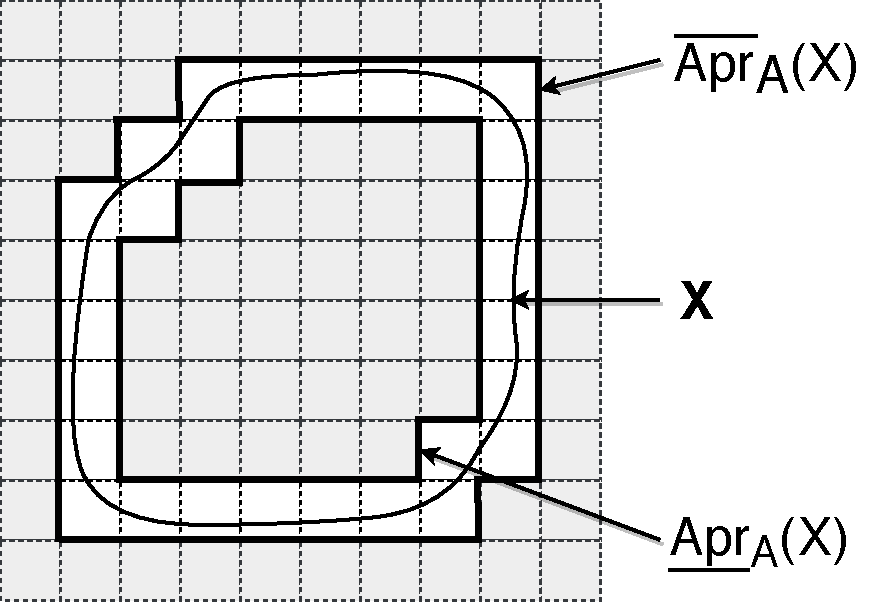
\includegraphics[width=0.75\textwidth]{Imagens/rought_set.pdf}
	\caption[Rought set approximation by lower and upper crisp sets]{Best approximation of the rough set $X$ by lower $B_{*}(X)$ and upper $B^{*}(X)$ crisp sets. The elementary granules are squares and the union of these granules form the universe of objects.}
	\label{fig:rough}
\end{figure}

In \citep{Pawlak1991} and in the references therein, many real life applications of rough set theory are explored, such as civil engineering, medical data analysis, aircraft pilot performance evaluation, vibration analysis and image processing.


\begin{table}[!htb]
	% increase table row spacing, adjust to taste
	\renewcommand{\arraystretch}{1.3}
	% if using array.sty, it might be a good idea to tweak the value of
	% \extrarowheight as needed to properly center the text within the cells
	\caption[Data fusion methods for imperfect data]{Data fusion methods for imperfect data, adapted from \citep[page 35, Table 1]{Khaleghi2013}}
	\label{tab:methods}
	\centering
	% Some packages, such as MDW tools, offer better commands for making tables
	% than the plain LaTeX2e tabular which is used here.
	\begin{flushleft}
	
	{
		\footnotesize
		\begin{tabularx}{\linewidth}{ 	>{\hsize=0.75\hsize}X
										>{\hsize=1.25\hsize}X
										>{\hsize=1.1\hsize}X
										>{\hsize=0.9\hsize}X}
			\hline
			\textbf{Algorithm} 			& \textbf{Approach}    			&  \textbf{Advantages} 		& \textbf{Limitations}\\ 
			\hline
			Probabilistic & Bayesian framework to fuse uncertain data represented by probability density functions & Well-established and optimal for certain conditions & Might be unsuited for other data imperfections \\ \\			
			Evidential Belief & Data fusion based on probability mass function, using Dempster-Shafer theory and combination rules & Enables fusion of both uncertain and ambiguous information & Incapable of dealing with other aspects of imperfection \\ \\ 
			Fuzzy Reasoning & Vague data represented by fuzzy set theory and fusion based on fuzzy rules & Intuitive and interpretable approach for vague data, such as human generated & Only applicable to vague data \\ \\
			Possibilistic & Data fusion based on fuzzy theory, with data representation similar to probabilistic and evidential belief & Indicated for poorly informed environment with incomplete data & Not very common and well-established \\ \\
			Rough Set & Imprecise data is approximated based on granularity and manipulated via classical set theory & Dispenses preliminary or additional information & Data granularity must be adequate \\ \\
			Random Set & Extension of Bayesian filter, representing the state space as a random set to capture many aspects of imperfection & Can potentially provide a unified framework for fusion of imperfect data & Not very appreciated by the fusion community \\ \\ 
			Hybridization & Combination of different fusion methods and data representation & More comprehensive treatment of data imperfection and benefits from complementary fusion & Computational expensive and very problem specific \\
		\end{tabularx}
	}
	\end{flushleft}

\end{table}


\section{Chapter Summary and Final Remarks}

In this chapter, sensor fusion literature is reviewed. We explore the discussion about performance improvement from the combination of information from multiple sources, that has been drawing attention for many decades. The main reasons for the evolution of sensor fusion as a field of science are presented in a comprehensive way, divided by the expected advantages in data authenticity and data availability. We continue with the definition and classification of sensor fusion approaches. Four main taxonomies are reviewed: classification based on sensor interaction; the input/output model based on the three fusion levels approach; sensor network architecture designs; and the categorization based on data challenge hierarchy. The last approach is especially interesting, since it relates to the core of this study: sensor fusion in the presence of irregularities in data. Algorithms that deal with the many aspects of data imperfection are summarized in Table~\ref{tab:methods}, such as: probabilistic; evidential belief; fuzzy logic; possibilistic; random set; and rough set theory. Hybrid methods have also being studied in the field, with interesting results.

Being the most popular method in the fusion community, the remaining of our study will focus on probabilistic methods for data fusion and its application on state estimation for sampled-data systems. A new data challenge is often present when complex sensor architectures are used to observe system states: sampling irregularity.


\clearpage